\documentclass[11pt,a4paper]{report}
\usepackage[textwidth=37em,vmargin=30mm]{geometry}
\usepackage{calc,xunicode,amsmath,amssymb,paralist,enumitem,tabu,booktabs,datetime2,xeCJK,xeCJKfntef,listings}
\usepackage{tocloft,fancyhdr,tcolorbox,xcolor,graphicx,eso-pic,xltxtra,xelatexemoji}

\newcommand{\envyear}[0]{2025}
\newcommand{\envdatestr}[0]{2025-08-12}
\newcommand{\envfinaldir}[0]{webdb/2025/20250812/final}

\usepackage[hidelinks]{hyperref}
\hypersetup{
    colorlinks=false,
    pdfpagemode=FullScreen,
    pdftitle={Web Digest - \envdatestr}
}

\setlength{\cftbeforechapskip}{10pt}
\renewcommand{\cftchapfont}{\rmfamily\bfseries\large\raggedright}
\setlength{\cftbeforesecskip}{2pt}
\renewcommand{\cftsecfont}{\sffamily\small\raggedright}

\setdefaultleftmargin{2em}{2em}{1em}{1em}{1em}{1em}

\usepackage{xeCJK,xeCJKfntef}
\xeCJKsetup{PunctStyle=plain,RubberPunctSkip=false,CJKglue=\strut\hskip 0pt plus 0.1em minus 0.05em,CJKecglue=\strut\hskip 0.22em plus 0.2em}
\XeTeXlinebreaklocale "zh"
\XeTeXlinebreakskip = 0pt


\setmainfont{Brygada 1918}
\setromanfont{Brygada 1918}
\setsansfont{IBM Plex Sans}
\setmonofont{JetBrains Mono NL}
\setCJKmainfont{Noto Serif CJK SC}
\setCJKromanfont{Noto Serif CJK SC}
\setCJKsansfont{Noto Sans CJK SC}
\setCJKmonofont{Noto Sans CJK SC}

\setlength{\parindent}{0pt}
\setlength{\parskip}{8pt}
\linespread{1.15}

\lstset{
	basicstyle=\ttfamily\footnotesize,
	numbersep=5pt,
	backgroundcolor=\color{black!5},
	showspaces=false,
	showstringspaces=false,
	showtabs=false,
	tabsize=2,
	captionpos=b,
	breaklines=true,
	breakatwhitespace=true,
	breakautoindent=true,
	linewidth=\textwidth
}






\newcommand{\coverpic}[2]{
    % argv: itemurl, authorname
    Cover photo by #2~~(\href{#1}{#1})
}
\newcommand{\makeheader}[0]{
    \begin{titlepage}
        % \newgeometry{hmargin=15mm,tmargin=21mm,bmargin=12mm}
        \begin{center}
            
            \rmfamily\scshape
            \fontspec{BaskervilleF}
            \fontspec{Old Standard}
            \fontsize{59pt}{70pt}\selectfont
            WEB\hfill DIGEST
            
            \vfill
            % \vskip 30pt
            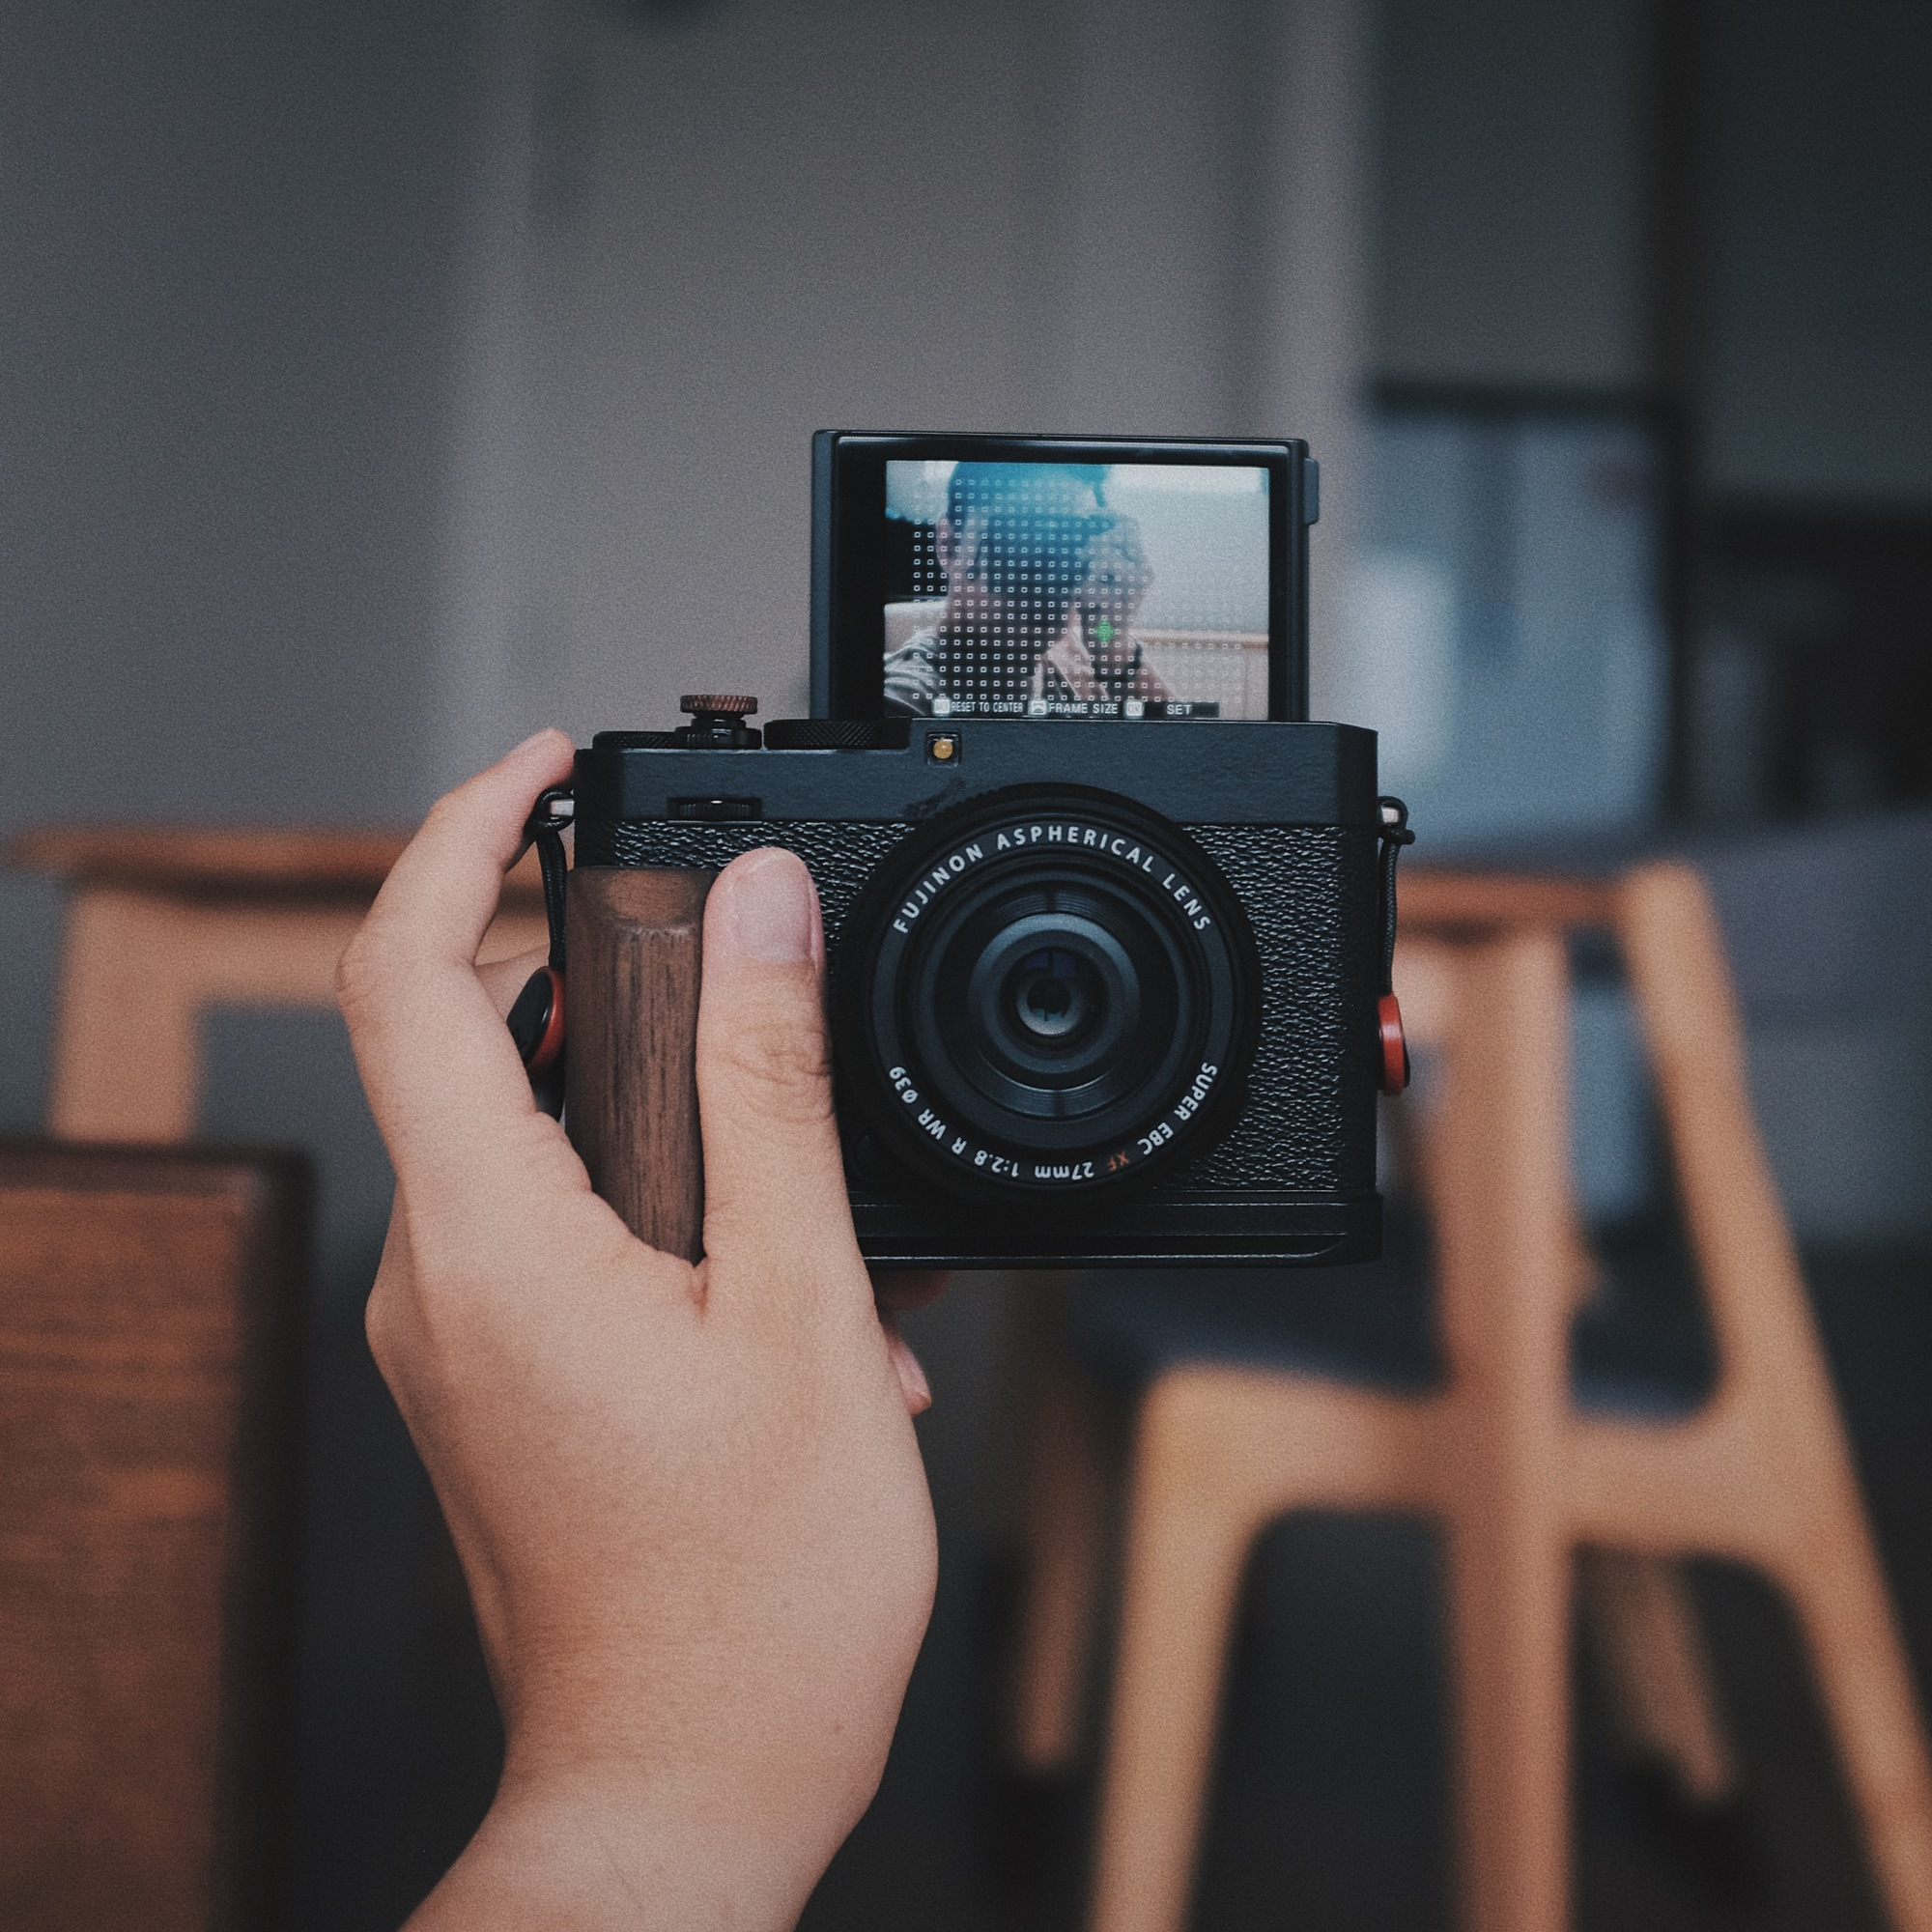
\includegraphics[width=\linewidth]{\envfinaldir/coverpic-prod.jpg}\par
            % \vskip 30pt
            \vfill

            \normalsize\rmfamily\scshape
            \copyright{} The Web Digest Project \hfill\large \envdatestr
        \end{center}
    \end{titlepage}
    % \restoregeometry
}
\newcommand{\simplehref}[1]{%
    \textcolor{blue!80!green}{\href{#1}{#1}}%
}
\renewcommand{\contentsname}{\center\Huge\sffamily\bfseries Contents\par\vskip 20pt}
\newcounter{ipartcounter}
\setcounter{ipartcounter}{0}
\newcommand{\ipart}[1]{
    % \vskip 20pt
    \clearpage
    \stepcounter{ipartcounter}
    \phantomsection
    \addcontentsline{toc}{chapter}{#1}
    % \begin{center}
    %     \Huge
    %     \sffamily\bfseries
    %     #1
    % \end{center}
    % \vskip 20pt plus 7pt
}
\newcounter{ichaptercounter}
\setcounter{ichaptercounter}{0}
\newcommand{\ichapter}[1]{
    % \vskip 20pt
    \clearpage
    \stepcounter{ichaptercounter}
    \phantomsection
    \addcontentsline{toc}{section}{\numberline{\arabic{ichaptercounter}}#1}
    \begin{center}
        \Huge
        \sffamily\bfseries
        #1
    \end{center}
    \vskip 20pt plus 7pt
}
\newcommand{\entrytitlefont}[1]{\subsection*{\raggedright\Large\sffamily\bfseries#1}}
\newcommand{\entryitemGeneric}[2]{
    % argv: title, url
    \parbox{\linewidth}{
        \entrytitlefont{#1}\par\vskip 5pt
        \footnotesize\ttfamily\mdseries
        \simplehref{#2}
    }\vskip 11pt plus 11pt minus 1pt
}
\newcommand{\entryitemGithub}[3]{
    % argv: title, url, desc
    \parbox{\linewidth}{
        \entrytitlefont{#1}\par\vskip 5pt
        \footnotesize\ttfamily\mdseries
        \simplehref{#2}\par\vskip 5pt
        \small\rmfamily\mdseries#3
    }\vskip 11pt plus 11pt minus 1pt
}
\newcommand{\entryitemAp}[3]{
    % argv: title, url, desc
    \parbox{\linewidth}{
        \entrytitlefont{#1}\par\vskip 5pt
        \footnotesize\ttfamily\mdseries
        \simplehref{#2}\par\vskip 5pt
        \small\rmfamily\mdseries#3
    }\vskip 11pt plus 11pt minus 1pt
}
\newcommand{\entryitemHackernews}[3]{
    % argv: title, hnurl, rawurl
    % \parbox{\linewidth}{
    %     \entrytitlefont{#1}\par\vskip 5pt
    %     \footnotesize\ttfamily\mdseries
    %     \simplehref{#3}\par
    %     \textcolor{black!50}{\href{#2}{#2}}
    % }\vskip 11pt plus 11pt minus 1pt
    \begin{minipage}{\linewidth}
            \entrytitlefont{#1}\par\vskip 5pt
            \footnotesize\ttfamily\mdseries
            \simplehref{#3}\par
            \textcolor{black!50}{\href{#2}{#2}}
    \end{minipage}\par\vskip 11pt plus 11pt minus 1pt
}







\begin{document}

\makeheader

\tableofcontents\clearpage




\ipart{Developers}
\ichapter{Hacker News}
\entryitemTwoLinks{I've seen 12 people hospitalized after losing touch with reality because of AI}{https://news.ycombinator.com/item?id=44869323}{https://twitter.com/KeithSakata/status/1954884361695719474}

\entryitemTwoLinks{Neki – sharded Postgres by the team behind Vitess}{https://news.ycombinator.com/item?id=44867374}{https://planetscale.com/blog/announcing-neki}

\entryitemTwoLinks{Token growth indicates future AI spend per dev}{https://news.ycombinator.com/item?id=44867312}{https://blog.kilocode.ai/p/future-ai-spend-100k-per-dev}

\entryitemTwoLinks{Wikipedia loses challenge against Online Safety Act}{https://news.ycombinator.com/item?id=44866208}{https://www.bbc.com/news/articles/cjr11qqvvwlo}

\entryitemTwoLinks{Claude is the drug, Cursor is the dealer}{https://news.ycombinator.com/item?id=44865813}{https://middlelayer.substack.com/p/i-claude-is-the-drug-cursor-is-the}

\entryitemTwoLinks{GitHub is no longer independent at Microsoft after CEO resignation}{https://news.ycombinator.com/item?id=44865560}{https://www.theverge.com/news/757461/microsoft-github-thomas-dohmke-resignation-coreai-team-transition}

\entryitemTwoLinks{Auf Wiedersehen, GitHub}{https://news.ycombinator.com/item?id=44864929}{https://github.blog/news-insights/company-news/goodbye-github/}

\entryitemTwoLinks{36B solar mass black hole at centre of the Cosmic Horseshoe gravitational lens}{https://news.ycombinator.com/item?id=44864680}{https://academic.oup.com/mnras/article/541/4/2853/8213862?login=false}

\entryitemTwoLinks{Meta Leaks Part 1: Israel and Meta}{https://news.ycombinator.com/item?id=44864419}{https://archive.org/details/meta\_leaks\_part\_1}

\entryitemTwoLinks{Trump Orders National Guard to Washington, D.C., and Takeover of City's Police}{https://news.ycombinator.com/item?id=44864192}{https://www.nytimes.com/live/2025/08/11/us/trump-news}

\entryitemTwoLinks{Claude Code is all you need}{https://news.ycombinator.com/item?id=44864185}{https://dwyer.co.za/static/claude-code-is-all-you-need.html}

\entryitemTwoLinks{I tried every todo app and ended up with a .txt file}{https://news.ycombinator.com/item?id=44864134}{https://www.al3rez.com/todo-txt-journey}

\entryitemTwoLinks{Wikimedia Foundation Challenges UK Online Safety Act Regulations}{https://news.ycombinator.com/item?id=44863487}{https://wikimediafoundation.org/news/2025/08/11/wikimedia-foundation-challenges-uk-online-safety-act-regulations/}

\entryitemTwoLinks{Pricing Pages – A Curated Gallery of Pricing Page Designs}{https://news.ycombinator.com/item?id=44863409}{https://pricingpages.design/}

\entryitemTwoLinks{OpenSSH Post-Quantum Cryptography}{https://news.ycombinator.com/item?id=44863242}{https://www.openssh.com/pq.html}

\entryitemTwoLinks{GPT-OSS-120B runs on just 8GB VRAM \& 64GB+ system RAM}{https://news.ycombinator.com/item?id=44862542}{https://old.reddit.com/r/LocalLLaMA/comments/1mke7ef/120b\_runs\_awesome\_on\_just\_8gb\_vram/}

\entryitemTwoLinks{Faster substring search with SIMD in Zig}{https://news.ycombinator.com/item?id=44862414}{https://aarol.dev/posts/zig-simd-substr/}

\entryitemTwoLinks{Hand-picked selection of articles on AI fundamentals/concepts}{https://news.ycombinator.com/item?id=44862112}{https://aman.ai/primers/ai/}

\entryitemTwoLinks{AOL to discontinue dial-up internet}{https://news.ycombinator.com/item?id=44861521}{https://www.nytimes.com/2025/08/11/business/aol-dial-up-internet.html}

\entryitemTwoLinks{The Chrome VRP Panel has decided to award \$250k for this report}{https://news.ycombinator.com/item?id=44861106}{https://issues.chromium.org/issues/412578726}


\ipart{Developers~~~~(zh-Hans)}
\ichapter{Solidot}
\entryitemGeneric{\hskip 0pt{}英伟达和 AMD 同意将 15\% 的中国营收上缴给美国}{https://www.solidot.org/story?sid=82008}

\entryitemGeneric{\hskip 0pt{}读卖新闻起诉 Perplexity 侵犯著作权}{https://www.solidot.org/story?sid=82006}

\entryitemGeneric{\hskip 0pt{}人与自然联结度 220 年来下降逾 60\%}{https://www.solidot.org/story?sid=82005}

\entryitemGeneric{\hskip 0pt{}安全加固的 Android 社区发行版 Graphene OS }{https://www.solidot.org/story?sid=82004}

\entryitemGeneric{\hskip 0pt{}Debian 13 trixie 释出}{https://www.solidot.org/story?sid=82003}

\entryitemGeneric{\hskip 0pt{}AI 淘汰初级编程开发者}{https://www.solidot.org/story?sid=82002}

\entryitemGeneric{\hskip 0pt{}签署捐赠誓言的 256 名亿万富翁只有 9 人信守诺言 }{https://www.solidot.org/story?sid=82001}

\entryitemGeneric{\hskip 0pt{}科学家研发能针对多种病毒的通用疫苗}{https://www.solidot.org/story?sid=82000}

\entryitemGeneric{\hskip 0pt{}Google 发现了一种新骗局,随后自己成为了该骗局的受害者}{https://www.solidot.org/story?sid=81999}

\entryitemGeneric{\hskip 0pt{}一颗大质量白矮星被发现是由双星合并而成}{https://www.solidot.org/story?sid=81998}

\entryitemGeneric{\hskip 0pt{}中国工程师解决磁悬浮列车的隧道微压波噪音}{https://www.solidot.org/story?sid=81997}\ichapter{V2EX}
\entryitemGeneric{\hskip 0pt{}[Solana] 主网币余额不足,请充值后再试}{https://www.v2ex.com/t/1151715}

\entryitemGeneric{\hskip 0pt{}[摄影] 有人在等理光 GR4 吗?}{https://www.v2ex.com/t/1151714}

\entryitemGeneric{\hskip 0pt{}[广州] 请问一下工作地点在广州石牌桥地铁站附近,希望能电驴半小时或者地铁半小时内到,有什么小区比较好呢?}{https://www.v2ex.com/t/1151713}

\entryitemGeneric{\hskip 0pt{}[macOS] macos26 beta6 刚升级完有什么变化吗?}{https://www.v2ex.com/t/1151712}

\entryitemGeneric{\hskip 0pt{}[分享创造] Google Chrome 内置 AI 啦,写了个完全在浏览器本地运行的翻译工具}{https://www.v2ex.com/t/1151711}

\entryitemGeneric{\hskip 0pt{}[问与答] 开源代码被人抄去用另一个语言重写闭源,只能认栽吗}{https://www.v2ex.com/t/1151709}

\entryitemGeneric{\hskip 0pt{}[分享创造] [开源] 做了个轻量自动化面板:实时 Token/费用监控 + 定时/智能调度}{https://www.v2ex.com/t/1151708}

\entryitemGeneric{\hskip 0pt{}[程序员] Hulo 编程语言开发 —— 从源代码到 AST 的魔法转换}{https://www.v2ex.com/t/1151707}

\entryitemGeneric{\hskip 0pt{}[问与答] 净水器换完滤芯,放进桶里两天就长青苔了,为啥啊?}{https://www.v2ex.com/t/1151706}

\entryitemGeneric{\hskip 0pt{}[宽带症候群] routeros 大佬都怎么玩的}{https://www.v2ex.com/t/1151705}

\entryitemGeneric{\hskip 0pt{}[问与答] 请问怎么才能解锁美亚账号}{https://www.v2ex.com/t/1151704}

\entryitemGeneric{\hskip 0pt{}[问与答] 如果你很轻松 50 万一年 会接受 6 万一个月事业单位的媳妇吗}{https://www.v2ex.com/t/1151701}

\entryitemGeneric{\hskip 0pt{}[分享创造] [开源] 又写了个无用的东西,但是有一点点好玩}{https://www.v2ex.com/t/1151700}

\entryitemGeneric{\hskip 0pt{}[Solana] 拥有 1000 V2EX 可以免费领服务器}{https://www.v2ex.com/t/1151698}

\entryitemGeneric{\hskip 0pt{}[酷工作] [社招] [深圳] 找个``靠谱''的 Web3 工作?持牌交易所,正在找 Java 大佬}{https://www.v2ex.com/t/1151697}

\entryitemGeneric{\hskip 0pt{}[问与答] 小米手机的满功率充电真的能达到吗?}{https://www.v2ex.com/t/1151696}

\entryitemGeneric{\hskip 0pt{}[问与答] 简历被反馈项目深度不够该怎么优化}{https://www.v2ex.com/t/1151695}

\entryitemGeneric{\hskip 0pt{}[加密货币] 加密货币提现的另一个选择 - 杜高思贝银行}{https://www.v2ex.com/t/1151694}

\entryitemGeneric{\hskip 0pt{}[问与答] 开通 github copilot, chatgpt 等是去办国内银行卡还是虚拟卡好}{https://www.v2ex.com/t/1151693}

\entryitemGeneric{\hskip 0pt{}[站长] GA 上显示流量突增是咋回事?}{https://www.v2ex.com/t/1151692}

\entryitemGeneric{\hskip 0pt{}[推广] 杭州联通各种优惠资费合计}{https://www.v2ex.com/t/1151691}

\entryitemGeneric{\hskip 0pt{}[宽带症候群] 上海移动 2000 兆三折来了华为 V271-20 尊享版设备}{https://www.v2ex.com/t/1151690}

\entryitemGeneric{\hskip 0pt{}[程序员] 使用 Claude Code 打造你的 AI 团队 (类似 Devin)}{https://www.v2ex.com/t/1151689}

\entryitemGeneric{\hskip 0pt{}[问与答] iPhone SE 升级困惑}{https://www.v2ex.com/t/1151688}

\entryitemGeneric{\hskip 0pt{}[反馈] 使用 Ledger 硬件钱包无法绑定 Solana 地址}{https://www.v2ex.com/t/1151686}

\entryitemGeneric{\hskip 0pt{}[Linux] Debian13 大家使用感觉如何}{https://www.v2ex.com/t/1151685}

\entryitemGeneric{\hskip 0pt{}[推广] 上海移动 2000 兆三折套餐重磅推出}{https://www.v2ex.com/t/1151684}

\entryitemGeneric{\hskip 0pt{}[问与答] ios safari 如何禁止打开某些网页强制跳转到 app, 比如百度,谷歌}{https://www.v2ex.com/t/1151683}

\entryitemGeneric{\hskip 0pt{}[问与答] 想入手一台 mac pro,求大佬推荐一下配置及性价比购买渠道;}{https://www.v2ex.com/t/1151682}

\entryitemGeneric{\hskip 0pt{}[问与答] 西昊 M59 Pro 和京东京造 Z9Pro 这两款电脑椅选哪个?}{https://www.v2ex.com/t/1151681}

\entryitemGeneric{\hskip 0pt{}[macOS] chatwise 快速定位到输入框的快捷键是什么?曲线方法用连按 tab 经常不成功。}{https://www.v2ex.com/t/1151680}

\entryitemGeneric{\hskip 0pt{}[Solana] 生成你的 V2EX(Solana)靓号钱包地址}{https://www.v2ex.com/t/1151679}

\entryitemGeneric{\hskip 0pt{}[酷工作] 七个座位,招募一起同行的构建者}{https://www.v2ex.com/t/1151678}

\entryitemGeneric{\hskip 0pt{}[问与答] 有用 n8n 真的改变生活的例子吗?}{https://www.v2ex.com/t/1151677}

\entryitemGeneric{\hskip 0pt{}[VXNA] 申请收录 https://www.xwenming.com}{https://www.v2ex.com/t/1151675}

\entryitemGeneric{\hskip 0pt{}[Solana] 蓝钻来了}{https://www.v2ex.com/t/1151673}

\entryitemGeneric{\hskip 0pt{}[问与答] Debian 13 关于 IP 转发的问题}{https://www.v2ex.com/t/1151672}

\entryitemGeneric{\hskip 0pt{}[问与答] 请教一下数据库相关的}{https://www.v2ex.com/t/1151671}

\entryitemGeneric{\hskip 0pt{}[分享发现] 免费奥地利手机号, Red Bull 送你,赶紧领起来}{https://www.v2ex.com/t/1151670}

\entryitemGeneric{\hskip 0pt{}[程序员] 在 vscode 中创建了一个分支,为什么显示了当前分支,又显示之前的分支?我只想显示当前分支}{https://www.v2ex.com/t/1151668}

\entryitemGeneric{\hskip 0pt{}[C] C11 的 \_Generic,现实当中用得多不多?(尤其是公司项目)}{https://www.v2ex.com/t/1151667}

\entryitemGeneric{\hskip 0pt{}[汽车] 日行灯还是很有必要的,毕竟有些人它不会开灯}{https://www.v2ex.com/t/1151666}

\entryitemGeneric{\hskip 0pt{}[问与答] Dropbox 不装代理软件该如何运行?}{https://www.v2ex.com/t/1151665}

\entryitemGeneric{\hskip 0pt{}[写周报] 独立开发周记 130: GPT-5 的表现出乎意料​}{https://www.v2ex.com/t/1151664}

\entryitemGeneric{\hskip 0pt{}[V2EX] 支付宝碰一下红包自动领取源码}{https://www.v2ex.com/t/1151663}

\entryitemGeneric{\hskip 0pt{}[问与答] 大学生毕业求建议}{https://www.v2ex.com/t/1151662}

\entryitemGeneric{\hskip 0pt{}[生活] 记一次归途中的晚霞}{https://www.v2ex.com/t/1151661}

\entryitemGeneric{\hskip 0pt{}[问与答] 支持流量付费,全球节点数量比较多且能用的机场,有推荐吗?}{https://www.v2ex.com/t/1151659}

\entryitemGeneric{\hskip 0pt{}[GitHub Copilot] Vscode 里 Copilot 调用 gemini api 失败}{https://www.v2ex.com/t/1151657}

\entryitemGeneric{\hskip 0pt{}[Android] 记一次一加 ace5 至尊版解锁和 root 过程}{https://www.v2ex.com/t/1151656}


\ipart{Generic News}







\clearpage
\leavevmode\vfill
\footnotesize

Copyright \copyright{} 2023-2025 Neruthes and other contributors.

This document is published with CC BY-NC-ND 4.0 license.

The entries listed in this newsletter may be copyrighted by their respective creators.

This newsletter is generated by the Web Digest project.

The newsletters are also delivered via Telegram channel \CJKunderline{\href{https://t.me/webdigestchannel}{https://t.me/webdigestchannel}}.\\
RSS feed is available at \CJKunderline{\href{https://webdigest.pages.dev/rss.xml}{https://webdigest.pages.dev/rss.xml}}.

This newsletter is available in PDF at
\CJKunderline{\href{https://webdigest.pages.dev/}{https://webdigest.pages.dev/}}.

The source code being used to generate this newsletter is available at\\
\CJKunderline{\href{https://github.com/neruthes/webdigest}{https://github.com/neruthes/webdigest}}.

This newsletter is also available in
\CJKunderline{\href{http://webdigest.pages.dev/readhtml/\envyear/WebDigest-20250812.html}{HTML}} and
\CJKunderline{\href{https://github.com/neruthes/webdigest/blob/master/markdown/\envyear/WebDigest-20250812.md}{Markdown}}.


\coverpic{https://unsplash.com/photos/palm-trees-reach-towards-a-vibrant-blue-sky-94xhfiXTkz4}{Fabio Sasso}


\end{document}
